\documentclass[12pt, reqno]{amsart}
% \pdfoutput=1



% Packages to open
\usepackage{amsthm, amssymb, amsmath, enumerate, textcomp}
% \usepackage{fullpage}
\usepackage{verbatim}
\usepackage{graphicx, graphics}
\usepackage{algorithm}
\usepackage{longtable}


% Setup TikZ

\usepackage{tikz}
\usetikzlibrary{arrows}
\tikzstyle{block}=[draw opacity=0.7,line width=1.4cm]

% Hopefully dot packages
\usepackage[all,arc,curve,frame,color]{xy}
\usepackage{subfigure}
\usepackage{url}








% \usepackage{setspace}  % Use command \doublespacing or \onehalfspacing

% Standard Theorem Styles
\newtheorem{thm}{Theorem}[section]
\newtheorem{lem}[thm]{Lemma}
\newtheorem{cor}[thm]{Corollary}
\newtheorem*{cor*}{Corollary}
\newtheorem{prop}[thm]{Proposition}
\newtheorem{obs}[thm]{Observation}
\newtheorem{claim}[thm]{Claim}
\newtheorem*{conjecture*}{Conjecture}
\newtheorem{conjecture}[thm]{Conjecture}
\newtheorem*{thm*}{Theorem}
\newtheorem{ps}{Problem Solving Strategy}

\theoremstyle{remark}
\newtheorem*{question*}{Question}
\newtheorem{question}[thm]{Question}
\newtheorem{answer}[thm]{Answer}
\newtheorem*{remark*}{Remark}
\newtheorem{example}[thm]{Example}
\newtheorem*{thinkpair*}{Think/Pair/Share}



\theoremstyle{definition}
\newtheorem{define}[thm]{Definition}
\newtheorem*{define*}{Definition}
\newtheorem{idea}{Idea}
\newtheorem{problem}{Problem}
\newtheorem{exercise}[thm]{Exercise}
\newtheorem*{problem*}{Problem}
\newtheorem*{sol*}{Solution}


\numberwithin{equation}{section}  % number equations by section

% Standard shortcuts
\newcommand{\LL}{\mathcal{L}}     % Fancy script L
\newcommand{\MM}{\mathcal{M}}  % Fancy script M
\newcommand{\OO}{\mathcal{O}}    % Fancy script O
\newcommand{\FF}{\mathbb{F}}      % Finite field
\newcommand{\ZZ}{\mathbb{Z}}     % Integers
\newcommand{\RR}{\mathbb{R}}     % Reals
\newcommand{\PP}{\mathbb{P}}      % Projective space
\newcommand{\Aff}{\mathbb{A}}      % Affine space
\newcommand{\XX}{\mathcal{X}}      % Model of a variety - script X
\newcommand{\QQ}{\mathbb{Q}}      %Rationals
\newcommand{\CC}{\mathbb{C}}      % Complex Numbers
\newcommand{\mm}{\mathfrak{m}}   % maximal ideal
\newcommand{\pp}{\mathfrak{p}}   % prime ideal
\newcommand{\qq}{\mathfrak{q}}  % another prime ideal
\newcommand{\Gm}{\mathbb{G}_m}  % blackboard bold G for the multiplicative group
\newcommand{\hh}{\mathfrak{h}}  % Upper half plane
\newcommand{\tab}{\hspace{.4cm}} % Tab 



 % Color comments!
\usepackage{xcolor}
% Color comments



%Notes to ourselves
\newcommand{\fellow}[1]{{\color{magenta} \sf $\clubsuit\clubsuit\clubsuit$ Fellow: [#1]}}
\newcommand{\michelle}[1]{{\color{blue} \sf $\clubsuit\clubsuit\clubsuit$ Michelle: [#1]}}


% Some regularly used operator shortcuts
\newcommand{\Hom}{\operatorname{Hom}}
\newcommand{\im}{\operatorname{im}} % Image
\newcommand{\coker}{\operatorname{coker}}  % Cokernel
\newcommand{\Sym}{\operatorname{Sym}}      % Symmetric product
\newcommand{\Spec}{\operatorname{Spec}}
\newcommand{\ord}{\operatorname{ord}}
\newcommand{\Div}{\operatorname{div}}    % Divisor of a rational function
\newcommand{\Gal}{\operatorname{Gal}}  % Galois group
\newcommand{\Gauss}{\operatorname{Gauss}}  % Used for the Gauss point
\newcommand{\supp}{\operatorname{supp}}   % Support
\newcommand{\Pic}{\operatorname{Pic}}        % Picard Groups
\newcommand{\Jac}{\operatorname{Jac}}       % Jacobian Variety
\newcommand{\mult}{\operatorname{mult}}  % multiplicity
\newcommand{\pr}{\operatorname{pr}}     % projection
\newcommand{\sep}[1]{{#1}^{\operatorname{s}}}    % separable closure
\newcommand{\Spf}{\operatorname{Spf}}    % formal spectrum
\newcommand{\Frac}{\operatorname{Frac}}    % Fraction field
\newcommand{\chern}[1]{c_1\left(#1\right)}   % First Chern class
\newcommand{\codim}{\operatorname{codim}}  % codimension
\newcommand{\dist}{\operatorname{dist}}   % distance
\newcommand{\an}[1]{\operatorname{an}}  % analytic space notation
\newcommand{\Aut}{\operatorname{Aut}}   % Automorphism group
\newcommand{\Rat}{\operatorname{Rat}}    % space of rational maps
\newcommand{\PGL}{\operatorname{PGL}}
\newcommand{\PSL}{\operatorname{PSL}}
\newcommand{\alg}[1]{{\overline{#1}}}
\newcommand{\GG}{\mathbb{G}}


% Miscellaneous notational shortcuts
\newcommand{\leftexp}[2]{{\vphantom{#2}}^{#1}{#2}}   % Superscript on the left
\newcommand{\simarrow}{\stackrel{\sim}{\rightarrow}}    % Isomorphic mapping
\newcommand{\ip}[2]{\left\langle #1,#2 \right\rangle} %inner product
\newcommand{\into}{\hookrightarrow}     % Inclusion arrow
\newcommand{\dint}{\int \!\!\! \int}   % double integral
\newcommand{\tth}{^{\operatorname{th}}}
\newcommand{\Berk}{\mathbf{P}}  % Berkovich Projective Space

\newcommand{\Manoa}{M\=anoa}
\newcommand{\Hawaii}{Hawai\kern.05em`\kern.05em\relax i}


% Document Specific Declarations
\newcommand{\id}{\mathrm{id}}
\newcommand{\oo}{\mathfrak{o}}
\DeclareMathOperator{\Per}{Per}
\DeclareMathOperator{\PrePer}{PrePer}
\DeclareMathOperator{\Twist}{Twist}
\DeclareMathOperator{\Ker}{Ker}


%%%%%%%%%%%%%%

\title{Chapter 1: Patterns and \\
Algebraic Thinking}

%%%%%%%%%%%%%%


\begin{document}


\maketitle

Algebra skills are essential for your future students.  Why?  Here are just a few reasons:
\begin{itemize}
\item
Mathematics, and especially algebra, is the language of  science and modern technology.  Thinking algebraically helps you to make sense of the world, to understand and interact with technology  more productively, and to succeed in other fields.

\item
Algebra is a tool for solving problems.  This may not be your experience so far, but it is true.  If you are able to ``algebratize'' a problem, that often helps lead you to a solution.

\item
Algebra helps you to think abstractly.  It is a tool for thinking about operations like addition, subtraction, multiplication, and division separate from doing calculations on numbers.  Algebra helps you to understand and explain why the operations work the way they do, to describe their properties clearly, and to manipulate expressions to see the bigger picture.

\end{itemize}


You might wonder why future elementary teachers should master algebra, a topic usually studied (by that name, anyway) in 8th grade and beyond.  But the Common Core Standards for School Mathematics\footnote{\url{http://www.corestandards.org/Math/Content/OA}} has standards in ``Operations and Algebraic Thinking'' beginning in kindergarten!

Everyone who shows up to school has already learned a lot about abstraction and generalization --- the fundamental ideas in algebra.  They are all capable of learning to formalize these ideas.  Your job as an elementary school teacher will be to provide your students with even more experiences in abstraction and generalization in a mathematical context, so that these ideas will seem quite natural when they get to a class with the name ``Algebra.''

\newpage

Let's start with a problem:
\begin{problem}\label{prob: four4s}
I can use four 4's to make 0:
\[
44 - 44 = 0.
\]
I can also use four 4's to make the number 10:
\[
(4 \times 4) - 4 - \sqrt 4 = 10.
\]

Your challenge: Use four 4's to make all of the numbers between 0 and 20.  (Try to find different solutions for 0 and 10 than the ones provided.)
You can use any mathematical operations, but you can't use any \emph{digits} other than the four 4's.
\end{problem}

\bigskip
\bigskip

\begin{thinkpair*}
Share your answers to Problem~\ref{prob: four4s} with a partner.  Then talk about these questions together:
\begin{itemize}
\item
What does ``algebra'' mean to you?  \\
\item
What does Problem~\ref{prob: four4s}  have to do with ``algebra''?\\
\item
What do you imagine when you think about using algebra to solve problems in school?  \\
\item
Have you ever used algebra to solve problems outside of school?\\
\item
What is meant by ``algebraic thinking,'' and what kinds of algebraic thinking can be done by elementary school students?
\end{itemize}
\end{thinkpair*} 

\newpage



\section{Borders on a Square}
Here's another problem.


\begin{problem}\label{prob: border}
Here is a large square made up of $100$ smaller unit squares.  The unit squares along the border of the large square are colored red.  Without counting one-by-one, can you figure out how many red squares there are in the picture?
Clearly describe how you figured out the number of red squares, and how you know your answer is correct.

\bigskip
\bigskip


\begin{center}
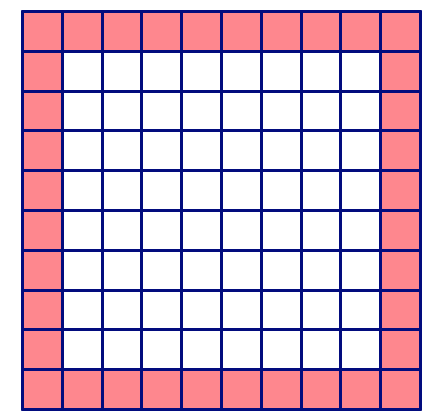
\includegraphics[height=5cm]{border1}
\end{center}
\end{problem}

\bigskip

\newpage

Justin calculated the number of squares as $(10 \times 4) - 4$.  He justified his answer this way:
\begin{quotation}
\emph{Since the dimensions of the big square are $10 \times 10$, there are $10$ squares along each of the four sides.  So that gives me $10 \times 4$ red squares.  But then each corner is part of two different sides.  I've counted each of the corners twice.  So I need to make up for that by subtracting $4$ at the end.}
\end{quotation}

Justin showed this picture to justify his work.
\begin{center}
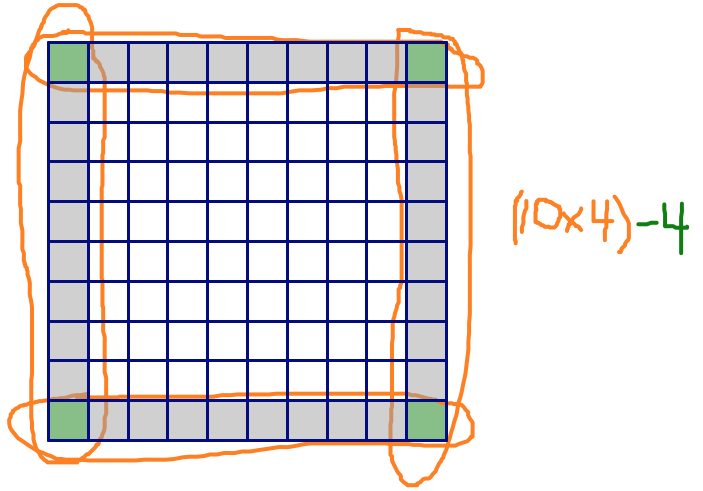
\includegraphics[height=6cm]{border2}
\end{center}

\bigskip
\bigskip


\begin{thinkpair*}
Discuss these questions with your partner:
\begin{itemize}
\item
What do you think about Justin's solution?  Are you convinced?  Could he have explained it more clearly?\\

\item
Was Justin's solution different from your solution or the same?  Discuss Justin's solution and your own solution with a partner.\\

\item
Notice the color coding in Justin's picture.  What do the colors represent?  Why did he use the colors the way he did?\\
\end{itemize}
\end{thinkpair*}

\newpage

\begin{problem}
There are lots of different ways to calculate the number of colored squares along the border of a $10\times 10$ square.  Below are the calculations several other students did.  For each calculation, write a justification and draw a picture to show why it calculates the number of squares correctly.  Think about using color in your picture to make your work more clear.

\begin{enumerate}[(a)]
\item
Valerie calculated $10 + 10 + 8 + 8$.\\

\item
Kayla calculated $4 \times 9$.\\


\item
Linda calculated $(10\times 10 ) - ( 8 \times 8 )$.\\

\item
Mark calculated $(4 \times 8) + 4$.\\

\item
Allan calculated $10+9+9+8$.
\end{enumerate}

\end{problem}


\bigskip



\begin{problem}
Now suppose that  you have a  large $6 \times 6$ square with the unit squares along the border  colored red.  Adapt two of the techniques above to calculate the number of red unit squares.
  For each technique you used, write an explanation and include a picture.  Think about how to use colors or other methods to make your picture and explanation more clear.
  \end{problem}
  
  \bigskip
  
  \begin{problem}
Now suppose that  you have a  large $25 \times 25$ square with the unit squares along the border  colored red.  Adapt two of the techniques above to calculate the number of red unit squares.
  For each technique you used, write an explanation and include a picture.  Think about how to use colors or other methods to make your picture and explanation more clear.
  \end{problem}

\bigskip

\begin{problem}\ 
\begin{enumerate}[(a)]
\item
Suppose that you have 64 red squares.  Can you use all of those squares to make the border of a larger square in a picture like the one above?  If yes, what are the dimensions of the larger square?  If no, why not?\\
\item
What if you have 30 red squares?  Same questions.\\
\item
What if you have 256 red squares?  Same questions.\\
\end{enumerate}
\end{problem}

\bigskip


\begin{thinkpair*}
With a partner, see if you can describe some general rules:
\begin{itemize}
\item
If you have a large $n \times n$ square with the border squares colored red, how many red squares will there be?  Justify your answer with words and a picture.\\

\item
If you have $k$ red squares, is there a quick test you can do to decide if you can use all of those squares to make the border of a large square?  Can you tell how big the square will be?
\end{itemize}
\end{thinkpair*}

\newpage




\section{Careful use of language in mathematics: $=$}
You have already thought about the careful use of language in mathematics.  For example, the word ``or'' has very specific meanings in math that is slightly different from their everyday use.

The notion of equality is fundamental in mathematics, and especially in algebra and algebraic thinking.  The symbol ``='' expresses a \emph{relationship}.  It is \emph{not} an operation in the way that $+$ and $\div$ are operations.  It should not be read left-to-right, and it definitely does not mean ``\dots and the answer is \dots''.


For your work to be clear and easily understood by others, it is essential that you use the symbol $=$ appropriately.  And for your future students to understand the meaning of the $=$ symbol and use it correctly, it is essential that you  are clear and precise in your use of it.

Let's start by working on some problems.

\begin{problem}\label{prob: grandma}
Akira went to visit his grandmother, and she gave him \$1.50 to buy a treat.
He went to the store and bought a book for \$3.20.   After that, he had \$2.30 left.
How much money did Akira have before he visited his grandmother?
\end{problem}

\bigskip

\begin{problem}\label{prob: equations}
Examine the following equations.  Decide: Is the statement always true, sometimes true, or never true?  Justify your answers.
\begin{align*}
(a) &\ 5 + 3 = 8.
&
(b) &\ \frac 23 + \frac 12 = \frac 35.
&
(c) & \ 5 + 3 = y.
& (d)& \ 
\frac a 5 = \frac 5 a.
\\
\\
(e) & \ n + 3 = m.
&
(f) & \ 3x = 2x + x.
&
(g)& \ 
5k = 5k + 1.
\end{align*}


\end{problem}

\bigskip


\begin{problem}\label{prob: equations2}
Consider the equation
\[ 
18 - 7 = \underline{\phantom{blah}}.
\]

\begin{enumerate}[(a)]
\item
Fill in the blank with something that makes the equation \emph{always true}.\\
\item
Fill in the blank with something that makes the equation \emph{always false}.\\
\item
Fill in the blank with something that makes the equation \emph{sometimes true and sometimes false}.
\end{enumerate}
\end{problem}



\bigskip


\begin{problem}
If someone asked you to \emph{solve} the equations in Problem~\ref{prob: equations}, what would you do in each case and why?
\end{problem}



\bigskip
\bigskip


\begin{thinkpair*}
Kim solved Problem~\ref{prob: grandma} this way this way:

\begin{quote}
\emph{
Let's see:
\[
2.30 + 3.20 = 5.50 - 1.50 = 4, 
\]
 so the answer is $4$.}
\end{quote}
What do you think about Kim's solution?  Did she get the correct answer?  Is her solution clear?  How could it be better?
\end{thinkpair*}

\bigskip
\bigskip

Although Kim found the correct numerical answer, her calculation really doesn't make any sense.  It is true that
\[
2.30 + 3.20 = 5.50.
\]
It is definitely not true that 
\[
2.30 + 3.20 = 5.50 - 1.40.
\]
She is incorrectly using the symbol ``='', and that makes her calculation hard to understand.  


\bigskip
\bigskip

\begin{thinkpair*}\ 
\begin{itemize}
\item
Can you write a good \emph{definition} of the symbol ``$=$''?  What does it mean and what does it represent?  \\

\item
Give some examples: When should the symbol ``$=$'' be used, and when should it \emph{not} be used?\\

\item
Do these two equations express the same relationships or different relationships?  Explain your answer.
\begin{align}
x^2 - 1 & = (x+1)(x-1)\\
(x+1)(x-1)  & = x^2 - 1
\end{align}\\

\end{itemize}
\end{thinkpair*}

\bigskip


This picture shows a (very simplistic) two-pan balance scale.  Such a scale allows you to \emph{compare} the weight of two objects.  Place one object in each pan.  If one side is lower than the other, then that side holds heavier objects.  If the two sides are balanced, then the objects on each side weigh the same.

\begin{center}
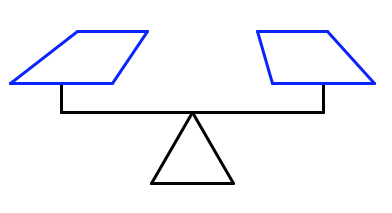
\includegraphics[height=2.8cm]{emptyscale}
\end{center}

\bigskip


\begin{thinkpair*}
In the pictures below:
\begin{itemize}
\item
The orange triangles all weigh the same.  
\item
The green circles all weigh the same.  
\item
The purple squares all weigh the same.  
\item
The silver stars all weigh the same.
\item
The scale is balanced.
\end{itemize}

\begin{center}
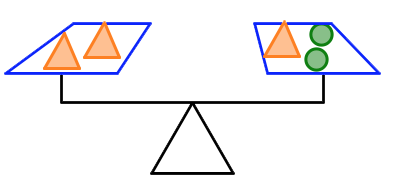
\includegraphics[height=3cm]{balancetalk1}\\
(a) What do you know about the weights of the triangles and the circles?  How do you know it?

\bigskip

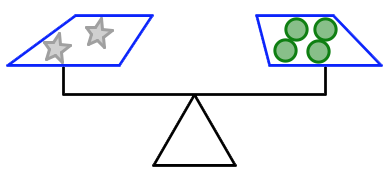
\includegraphics[height=3cm]{balancetalk2}\\
(b) What do you know about the weights of the circles and the stars?  How do you know it?

\bigskip

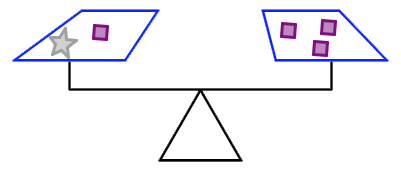
\includegraphics[height=3cm]{balancetalk3}\\
(c) What do you know about the weights of the stars and the squares?  How do you know it?


\end{center}



\end{thinkpair*}

\bigskip

\begin{problem}\label{prob: balance1}
In the pictures below:
\begin{itemize}
\item
The orange triangles all weigh the same.  
\item
The green circles all weigh the same.  
\item
The purple squares all weigh the same.  
\item
The scale is balanced.
\end{itemize}
How many purple squares will balance with one circle?  Justify your answer.
\begin{center}
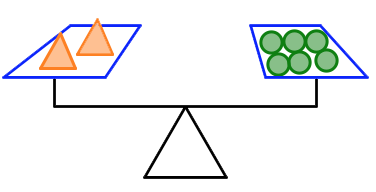
\includegraphics[height=3cm]{balance1a}\quad
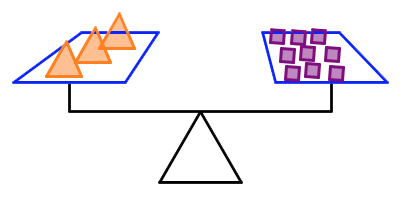
\includegraphics[height=3cm]{balance1b}

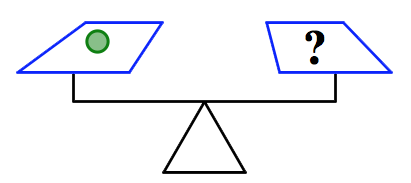
\includegraphics[height=3cm]{balance1c}

\end{center}

\end{problem}

\bigskip

\begin{problem}\label{prob: balance2}
In the pictures below:
\begin{itemize}
\item
The orange triangles all weigh the same.  
\item
The green circles all weigh the same.  
\item
The purple squares all weigh the same.  
\item
The silver stars all weigh the same.
\item
The scale is balanced.
\end{itemize}
How many purple squares will balance the scale in each case?  Justify your answers.
\begin{center}
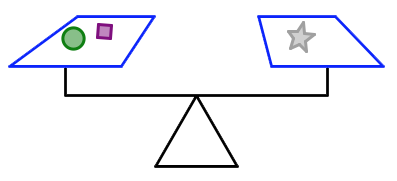
\includegraphics[height=2.7cm]{balance2a}\quad
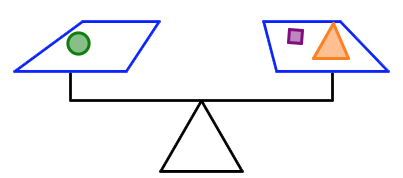
\includegraphics[height=2.7cm]{balance2b}
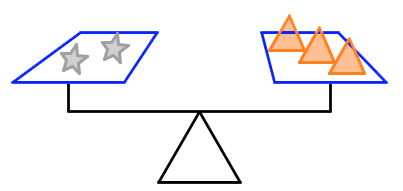
\includegraphics[height=2.7cm]{balance2c}

\bigskip
\bigskip

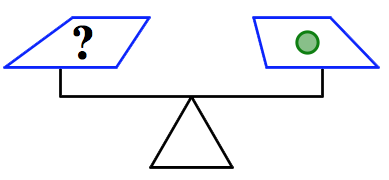
\includegraphics[height=3cm]{balance2d1}\\
(a)

\bigskip

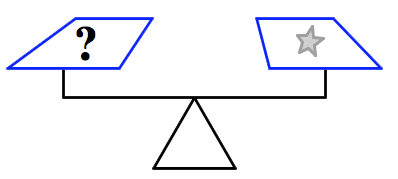
\includegraphics[height=3cm]{balance2d2}\\
(b)
\bigskip


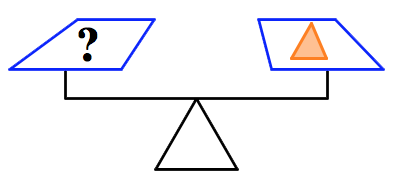
\includegraphics[height=3cm]{balance2d3}\\
(c)

\end{center}

\end{problem}


\newpage


\begin{problem}\label{prob: balance3}
In the pictures below:
\begin{itemize}
\item
The orange triangles all weigh the same.  
\item
The green circles all weigh the same.  
\item
The purple squares all weigh the same.  
\item
The scale is balanced.
\end{itemize}
 What will balance the scale?  Can you find more than one answer?
\begin{center}
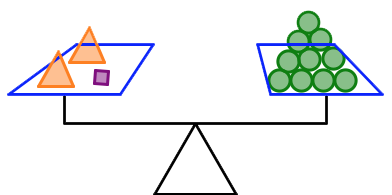
\includegraphics[height=2.7cm]{balance3a}\quad
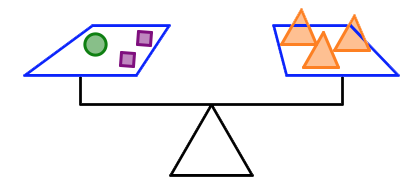
\includegraphics[height=2.7cm]{balance3b}

\bigskip

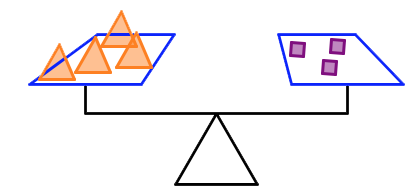
\includegraphics[height=2.7cm]{balance3c}\quad
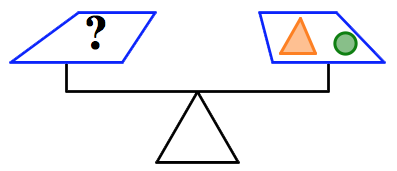
\includegraphics[height=2.7cm]{balance3d}

\end{center}

\end{problem}

\bigskip


\begin{problem}\label{prob: balance4}
In the pictures below:
\begin{itemize}
\item
The orange triangles all weigh the same.  
\item
The green circles all weigh the same.  
\item
The purple squares all weigh the same.  
\item
The scale is balanced.
\end{itemize}

\begin{center}
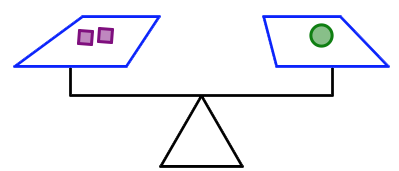
\includegraphics[height=2.6cm]{balance4a}\quad
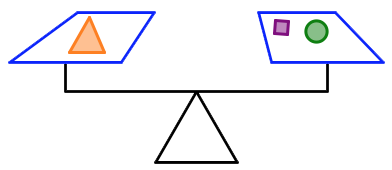
\includegraphics[height=2.6cm]{balance4b}

\end{center}

\begin{enumerate}[(a)]
\item
Which shape weighs the most: the square, the triangle, or the circle?  Which shape weighs the least?  Justify your answers.\\
\item
Which of the two scales is holding the most total weight?  How do you know you're right?
\end{enumerate}


\end{problem}





\bigskip
\bigskip

\bigskip

\begin{thinkpair*}
What do Problems~\ref{prob: balance1}--\ref{prob: balance4} above have to do with the ``$=$'' symbol?  
\end{thinkpair*}



\newpage

\section{Growing Patterns}
Here is a pattern made from square tiles.

\begin{center}
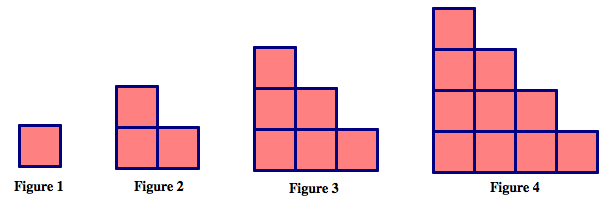
\includegraphics[height=5cm]{staircase}
\end{center}


\bigskip
\bigskip



\begin{thinkpair*}
First on your own and then with a partner, think about these questions:
\begin{itemize}
\item
Describe how you see this pattern growing.  Be as specific as you can.  Draw pictures and write an explanation to make your answer clear.\\

\item
Say as much as you can about this growing pattern.  Can you draw pictures to extend the pattern?  \\

\item
What mathematical questions can you ask about this pattern?  Can you answer any of them?\\
\end{itemize}
\end{thinkpair*}

\newpage

Here are some pictures that students drew to describe how the pattern was growing.  

\begin{center}
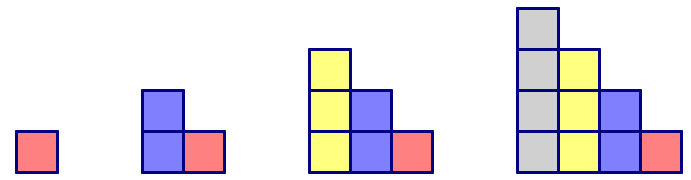
\includegraphics[height=3.5cm]{growth1}
Ali's picture.

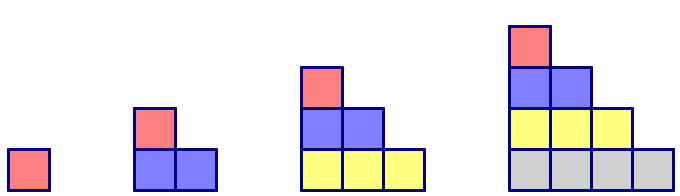
\includegraphics[height=3.5cm]{growth2}
Michael's picture.

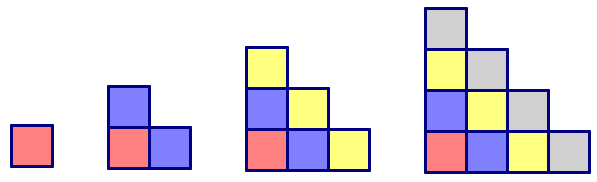
\includegraphics[height=3.5cm]{growth3}
Kelli's picture.

\end{center}


\bigskip


\begin{thinkpair*}
Describe in words how each student saw the pattern growing.
Use the students' pictures above (or your own method of seeing the growing pattern) to answer the following questions:
\begin{itemize}
\item
How many tiles would you need to build the 5th figure in the pattern?\\

\item
How many tiles would you need to build the 10th figure in the pattern?\\


\item
How can you compute the number of tiles in any figure in the pattern?
\end{itemize}

\end{thinkpair*}

\newpage


\begin{problem}
Hy saw the pattern in a different way from everyone else in class.  Here's what he drew:
\begin{center}
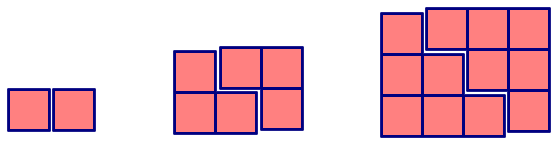
\includegraphics[height=3.5cm]{doubledstairs}
Hy's picture.
\end{center}
\begin{enumerate}[(a)]
\item
Describe in words how Hy saw the pattern grow.\\

\item
How would Hy calculate the number of tiles needed to build the 10th figure in the pattern?\\


\item
How would Hy calculate the number of tiles needed to build the 100th figure in the pattern?\\

\item
How would Hy calculate the number of tiles needed to build any figure in the pattern?
\end{enumerate}

\end{problem}

\newpage

The next few problems present several growing patterns made with tiles.  For each problem you work on, do the following:
\begin{enumerate}[(a)]
\item
Describe in words and pictures how you see the pattern growing.\\

\item
Calculate the number of tiles you would need to build the 10th figure in the pattern.  Justify your answer based on how the pattern grows.\\

\item
Calculate the number of tiles you would need to build the 100th figure in the pattern.  \\

\item
Describe how you can figure out the number of tiles in any figure in the pattern.  Be sure to justify your answer based on how the pattern grows.\\

\item
Could you make one of the figures in the pattern using exactly 25 tiles?  If yes, which figure?  If no, why not?  Justify your answer.\\

\item
Could you make one of the figures in the pattern using exactly 100 tiles?  If yes, which figure?  If no, why not?    Justify your answer.\\



\end{enumerate}

\bigskip

\begin{problem}\ 

\begin{center}
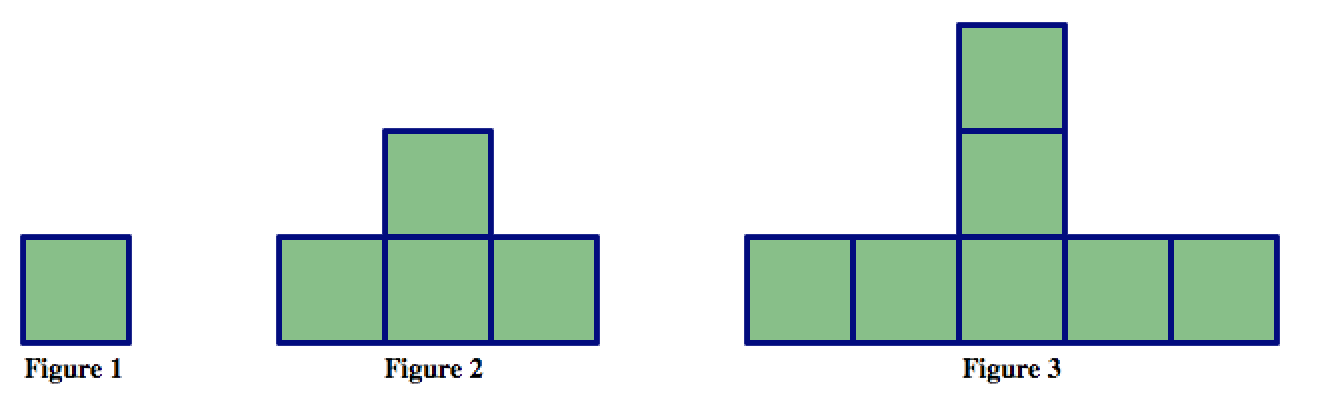
\includegraphics[height=4.25cm]{pattern2}
\end{center}

\end{problem}

\bigskip


\begin{problem}\ 

\begin{center}
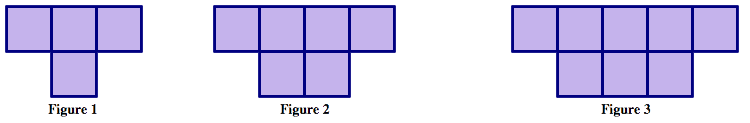
\includegraphics[height=2.5cm]{pattern3}
\end{center}

\end{problem}

\newpage

\begin{problem}\ 

\begin{center}
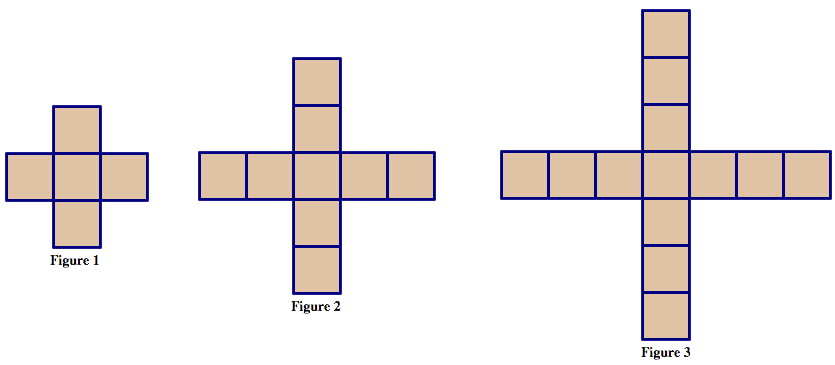
\includegraphics[height=6cm]{pattern4}
\end{center}

\end{problem}

\bigskip


\begin{problem}\ 

\begin{center}
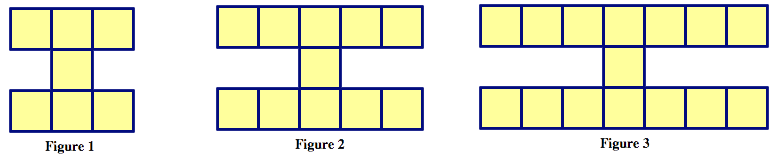
\includegraphics[height=3.25cm]{pattern5}
\end{center}

\end{problem}



\bigskip


\begin{problem}\ 

\begin{center}
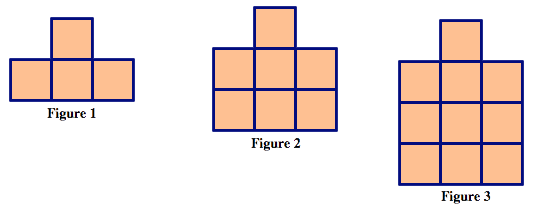
\includegraphics[height=4.5cm]{pattern6}
\end{center}

\end{problem}



\newpage





\section{Matching Game}\label{sec: matching}
Below, you'll find patterns described in various ways: through visual representations, algebraic expressions, in tables of numbers, and in words.  Your job is to match these up in a way that makes sense.    

 Note: there may be more than one algebraic expression to match a given pattern, or more than one pattern to match a given description.  So be ready to justify your answers.

\subsection*{Algebraic expressions}

\begin{align*}
(a) & \  t^2 
&
(b) & \  2s + 1 
&
(c) & \  2k + (k-1) + 2k + (k-1)
\\
\\
(d) & \  5n + 5
& 
(e) & \ a + a
& 
(f) & \ 3(\ell - 1) + 3 (\ell - 1) + 4
\\
\\
(g) & \  3b + 1
& 
(h) & \ z+ z+ 1
& 
(i) & \ m^2 - (m-1)^2
\\
\\
(j) & \  y\cdot y
& 
(k) & \  2x - 1
& 
(\ell) & \ 4e - (e-1)
\\
\\
(m) & \  6f - 2
& 
(n) & \  2c
& 
(o) & \ 5(s+1)
\end{align*}


\bigskip
\bigskip

\subsection*{Visual patterns}

\begin{center}
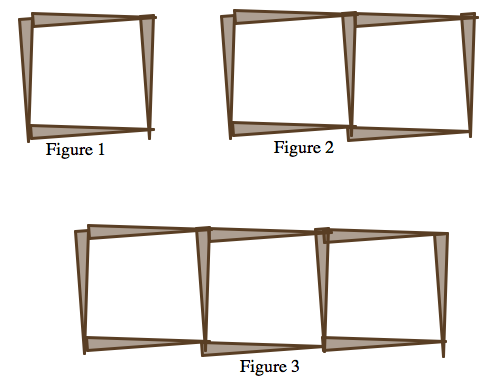
\includegraphics[height=6cm]{matching1}\\
Pattern 1

\bigskip


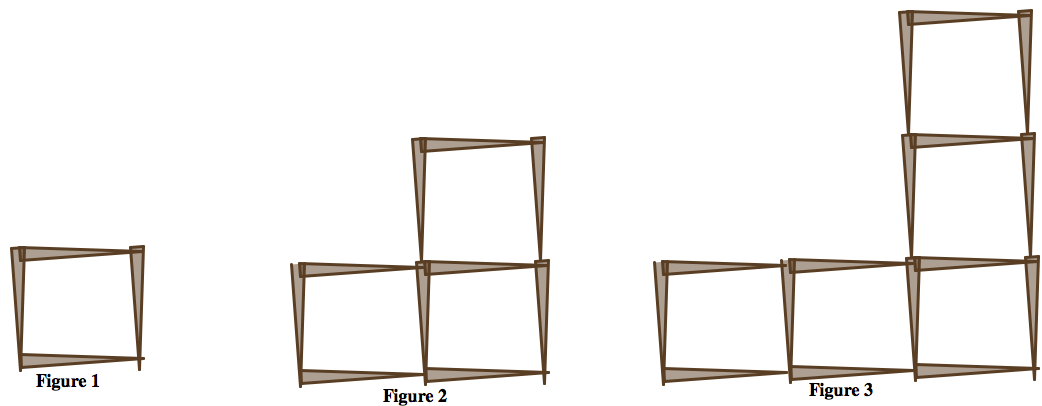
\includegraphics[height=6cm]{matching2}\\
Pattern 2


\bigskip

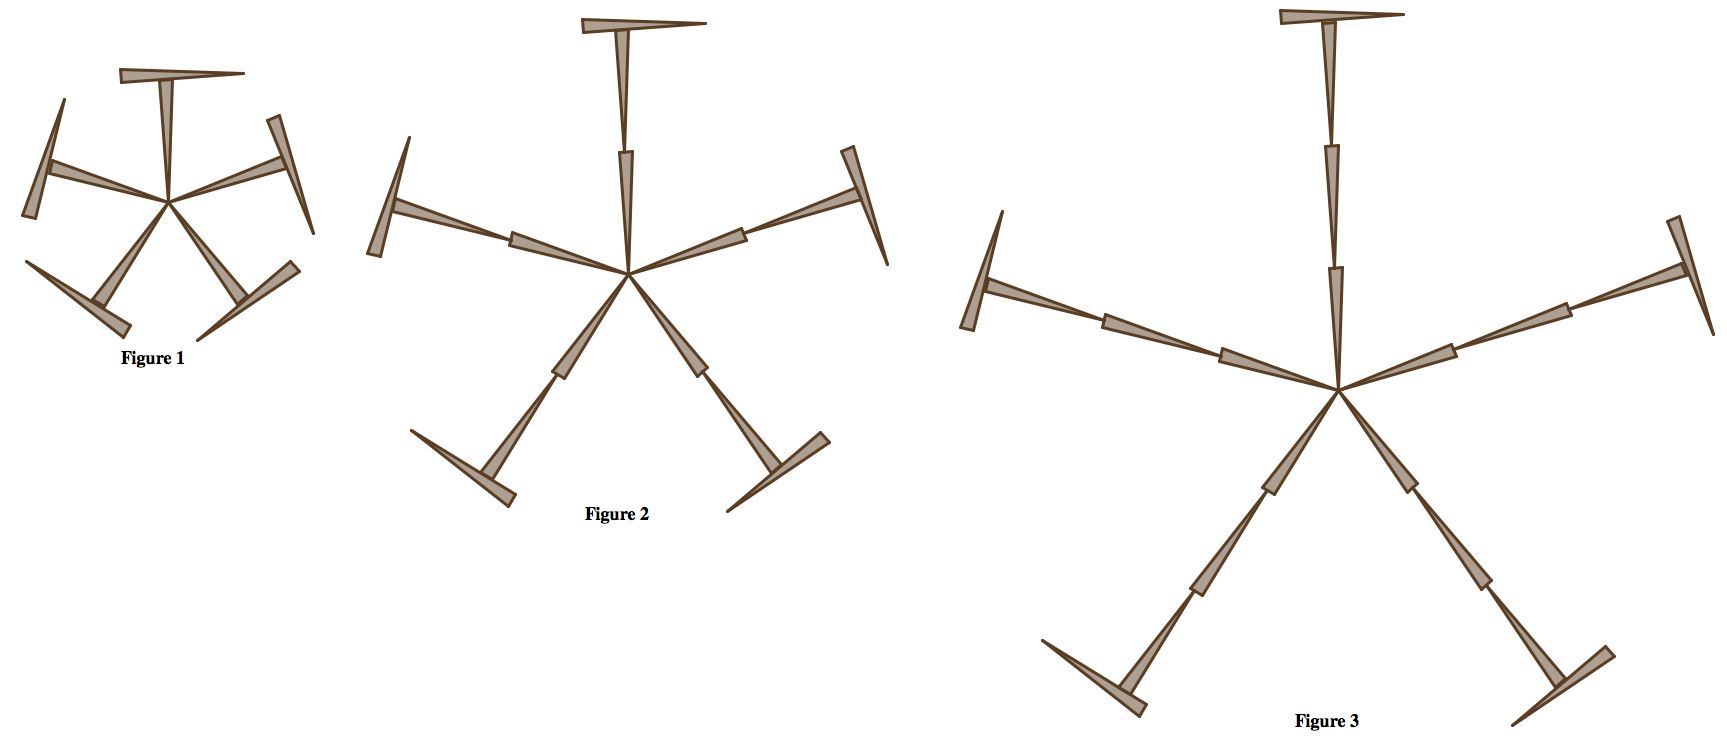
\includegraphics[height=7cm]{matching3}\\
Pattern 3


\bigskip

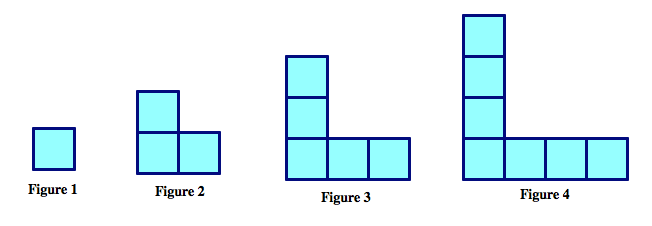
\includegraphics[height=5cm]{matching4}\\
Pattern 4

\bigskip

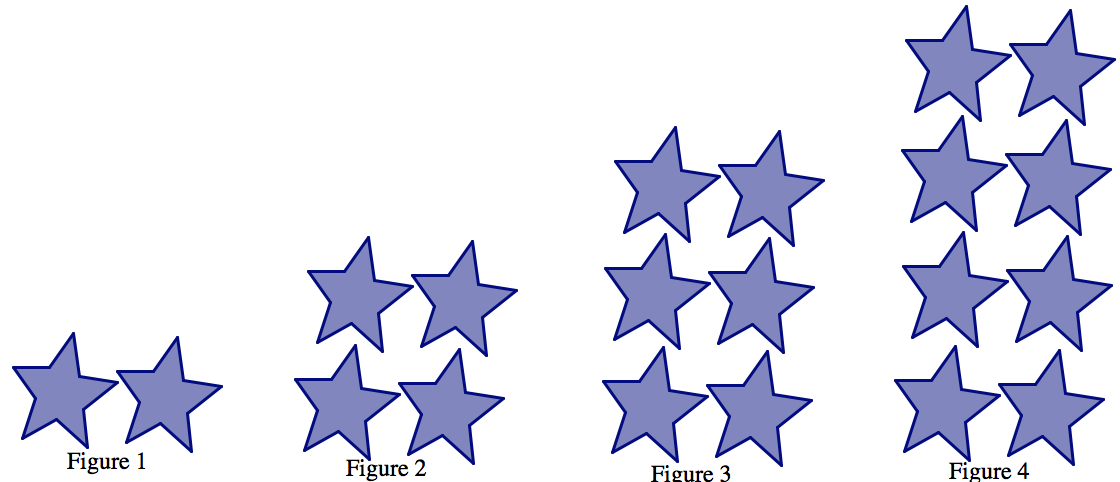
\includegraphics[height=6cm]{matching5}\\
Pattern 5

\bigskip

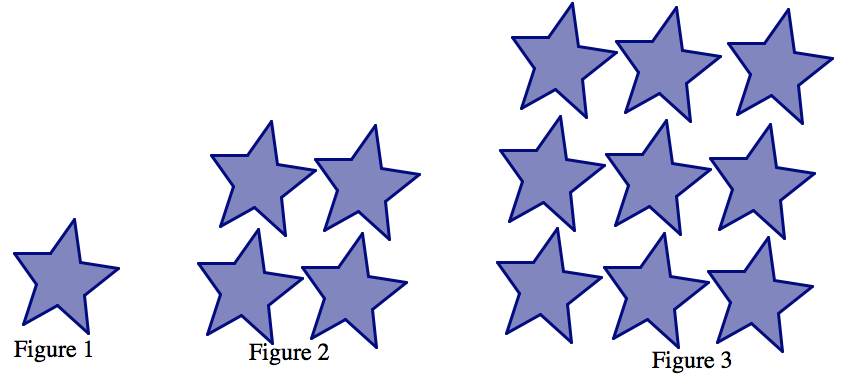
\includegraphics[height=5cm]{matching6}\\
Pattern 6

\bigskip

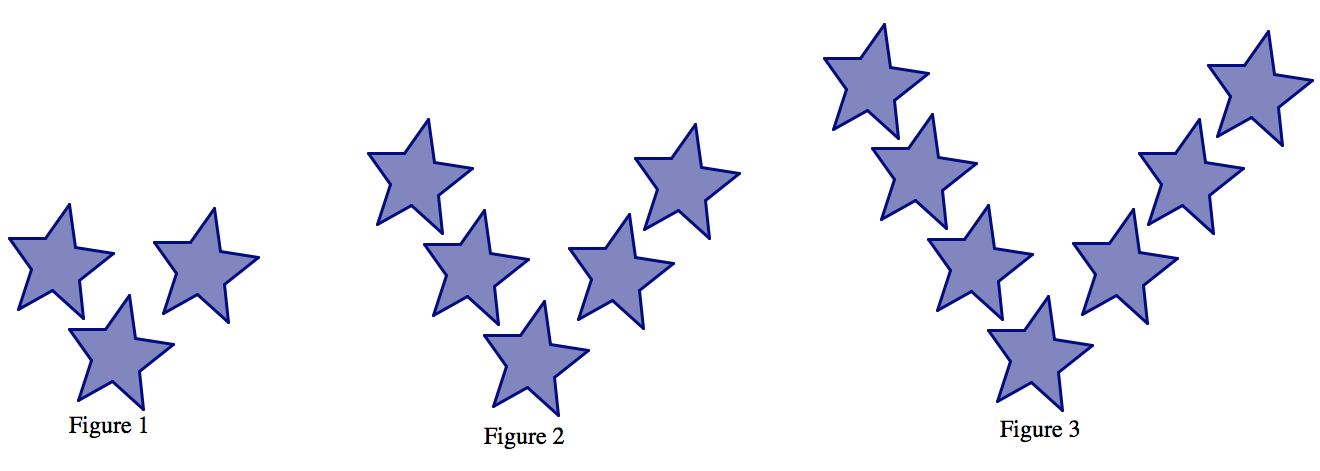
\includegraphics[height=5.5cm]{matching7}\\
Pattern 7


\end{center}


\bigskip
\bigskip


\subsection*{Tables of Numbers}\ 

\begin{center}

\begin{tabular}{c || c | c | c | c }
\multicolumn{5}{c}{Table A}\\
Input \quad  & \quad  1 \quad & \quad  2  \quad & \quad  3  \quad & \quad 4  \quad \\\hline
Output \quad  & \quad  1 \quad & \quad  4  \quad & \quad  9  \quad & \quad 16  \quad 
\end{tabular}

\bigskip
\bigskip


\begin{tabular}{c || c | c | c | c }
\multicolumn{5}{c}{Table B}\\
Input \quad  & \quad  1 \quad & \quad  2  \quad & \quad  3  \quad & \quad 4  \quad \\\hline
Output \quad  & \quad  10 \quad & \quad  15  \quad & \quad  20  \quad & \quad 25  \quad 
\end{tabular}


\bigskip
\bigskip


\begin{tabular}{c || c | c | c | c }
\multicolumn{5}{c}{Table C}\\
Input \quad  & \quad  1 \quad & \quad  2  \quad & \quad  3  \quad & \quad 4  \quad \\\hline
Output \quad  & \quad  1 \quad & \quad  3  \quad & \quad  5  \quad & \quad 7  \quad 
\end{tabular}



\bigskip
\bigskip


\begin{tabular}{c || c | c | c | c }
\multicolumn{5}{c}{Table D}\\
Input \quad  & \quad  1 \quad & \quad  2  \quad & \quad  3  \quad & \quad 4  \quad \\\hline
Output \quad  & \quad  3 \quad & \quad  5  \quad & \quad  7  \quad & \quad 9  \quad 
\end{tabular}




\bigskip
\bigskip


\begin{tabular}{c || c | c | c | c }
\multicolumn{5}{c}{Table E}\\
Input \quad  & \quad  1 \quad & \quad  2  \quad & \quad  3  \quad & \quad 4  \quad \\\hline
Output \quad  & \quad  4 \quad & \quad  7  \quad & \quad  10  \quad & \quad 13  \quad 
\end{tabular}


\bigskip
\bigskip


\begin{tabular}{c || c | c | c | c }
\multicolumn{5}{c}{Table F}\\
Input \quad  & \quad  1 \quad & \quad  2  \quad & \quad  3  \quad & \quad 4  \quad \\\hline
Output \quad  & \quad  4 \quad & \quad  10  \quad & \quad  16  \quad & \quad 22  \quad 
\end{tabular}


\bigskip
\bigskip


\begin{tabular}{c || c | c | c | c }
\multicolumn{5}{c}{Table G}\\
Input \quad  & \quad  1 \quad & \quad  2  \quad & \quad  3  \quad & \quad 4  \quad \\\hline
Output \quad  & \quad  2 \quad & \quad  4  \quad & \quad  6  \quad & \quad 8  \quad 
\end{tabular}




\end{center}


\bigskip
\bigskip


\subsection*{Descriptions in words}

\begin{enumerate}[(i)]

\item
Count horizontal and vertical toothpicks separately.  Horizaontal: there are two rows of $n$ toothpicks where $n$ is the figure number.  There are $n-1$ more of them on the vertical arm.  The vertical toothpicks are just the same.  There are two colums of $n$ along the  vertical arm, and then $n-1$ more of them on the horizontal arm.\\



\item
 To get a figure from the previous one, you add three toothpicks in a ``C'' shape on the left side of the figure.  The total number of toothpicks is three times the figure number, plus one extra to close off the square on the far right.\\


\item
 There are five spikes radiating out from the center.  Each spike has the same number of toothpicks as the figure number.  Each spike is capped off by one additional toothpick.\\
 
 \item
Each arm of the ``L'' shape has the same number of tiles as the figure number.  But then we've counted the corner of the ``L'' twice, so we have to subtract one to get the total number of tiles needed.\\

\item
The stars are in two equal rows, and each row has the same number of stars as the figure number.\\

\item
To make the next figure, you always add five more toothpicks.  Each arm has one more than the figure number of toothpicks, and there are five arms.\\



\item
The stars are in a square, and the sides of the square have the same number of stars as the figure number.\\

\item
Each arm of the ``V'' shape has the same number of stars as the figure number.  Then we need to add one more star for the corner.\\


\item
There are the same number of squares as the figure number, and each square uses four toothpicks.  But then I've double-counted the toothpicks  where the squares touch, so we have to subtract those out.  There are one less of those than the figure number.\\

\newpage 

\item
I can picture a square of tiles filled in.  The side length of that square is the same as the figure number, so that's $x^2$.  But then the square isn't really filled in.  It's like I took away a square one size smaller from the top right, leaving just the border.  What I took away was a square one size smaller, $(x-1)^2$.\\

\item
Each time I go from one shape to the next, I add six new toothpicks.  Three are added to the left in a ``C'' shape and three are added to the top in a rotated ``C'' shape.  So the total number will be six times the figure number plus or minus something.  I can check to see that the right correction is to subtract 2.\\


\end{enumerate}




\newpage



\section{Structural and Procedural Algebra}
When most people think about algebra from school, they think about ``solving for $x$.''  They imagine lots of equations with varying levels of complexity, but the goal is always the same: find the unknown quantity.  This is a \emph{procedural} view of algebra.  

Even elementary students can  be exposed  ideas in procedural algebra.   This happens any time   they think about unknown quantities and try to solve for them.  For example, when first grade students learn to add and subtract numbers ``within 10,'' they should frequently tackle problems like these:

\begin{itemize}
\item
$3 + \underline{\qquad} = 7$.\\
\medskip
\item
Find several pairs of numbers that add up to 10.\\
\medskip
\end{itemize}

\bigskip

Although procedural algebra is important, it's not the most important skill, and it's certainly not the whole story.
You also need to foster thinking about  \emph{structural algebra} in your students: using symbols to express meaning in a situation.  If there is an $x$ on your page, you should be able to answer, ``what does the $x$ mean?  What does it represent?''  

Most of what you've done so far in this chapter is \emph{structural algebra}.  You've used letters and symbols not to represent a single unknown quantity, but a \emph{varying} quantity.  For example, in Section~\ref{sec: matching} you used letters to represent the ``figure number'' or ``case number'' in a growing pattern.  The letters could take on different values, and the expressions gave you information: how many tiles or toothpicks or stars you needed to build that particular figure in that particular pattern.

\newpage

\begin{thinkpair*}\ 
\begin{itemize}
\item
Consider the expression $a + 3$.  Give a real world situation that could be represented by this expression.  Share your answer with your partner.  Together, can you come up with even more ideas?\\
\item
Suppose the expression $3c+2$ represents the number of tiles used at any stage of a growing pattern. 
\begin{itemize}
\item
 Evaluate the expression at $c = 1, 2, \text{ and } 3$.  What do the values tell you about the pattern?  \\
 \item
 Can you describe in words how the pattern is growing?  \\
 \item
 Can you design a pattern with tiles that grows according to this rule?\\
 \item
 Where do you see the ``3'' from $3c+2$ in your pattern?  Where do you see the ``2''?  Where do you see the ``$c$''?
\end{itemize}
\end{itemize}
\end{thinkpair*}


\newpage

\begin{problem}\label{prob: krystal}
Krystal was looking at this pattern, which may be familiar to you from the Problem Bank:
\begin{center}
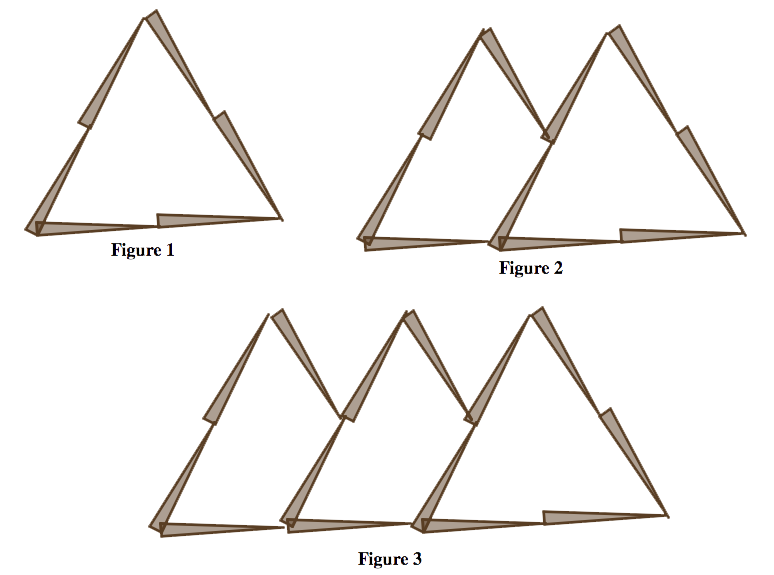
\includegraphics[height=8.5cm]{toothpicks4}
\end{center}
She wrote down the equation
\[
y = 4x + 2.
\]
In Krystal's equation, what does $x$ represent?  What does $y$ represent?  How do you know?


\end{problem}

\bigskip


\begin{problem}
Candice was thinking about this problem:
\begin{center}
\emph{Today is Jennifer's birthday, and she's twice as old as her brother.  When will she be twice as old as him again?}
\end{center}
She wrote down the equation $2 n = m$.  In Candice's equation, what does $n$ represent?  What does $m$ represent?  How do you know?

\end{problem}

\bigskip

\begin{problem}
Sarah and David collect old coins.  Suppose the variable $k$ stands for the number of coins Sarah has in her collection, and $\ell$ stands for the number of coins David has in his collection.  What would each of these equations say about their coin collections?

\[
(a)\  k = \ell + 1 
\qquad\qquad
(b)\  k = \ell 
\qquad\qquad
(c) \ 3k = 2\ell
\qquad\qquad
(d)\  k = \ell - 11
\]


\end{problem}



\bigskip


\begin{problem}\label{prob: bagsblocks}
The pictures below show balance scales containing bags and blocks.  The bags are marked with a ``?'' because they contain some unknown number of blocks.  In each picture:
\begin{itemize}
\item
Each bag contains the same number of blocks. 
\item
The scale is balanced.
\end{itemize}
For each picture, determine how many blocks are in each bag.  Justify your answers.

\begin{center}
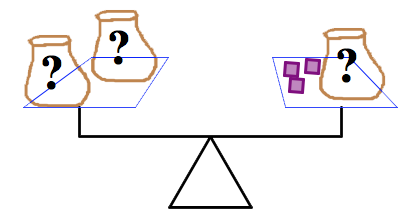
\includegraphics[height=3.5cm]{bags1}\\
(a)

\bigskip

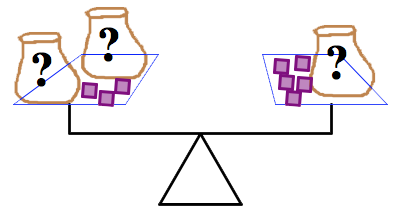
\includegraphics[height=3.5cm]{bags2}\\
(b)

\bigskip

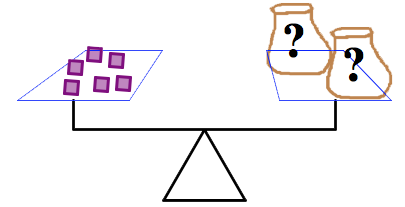
\includegraphics[height=3.5cm]{bags3}\\
(c)


\end{center}
\end{problem}


\bigskip

\begin{problem}
When he was working on Problem~\ref{prob: bagsblocks}, Kyle wrote down these three equations.  
\[
(i)\ 2m = 6.
\qquad
(ii)\ 2x = x + 3.
\qquad
(iii)\ z + 5 = 2z + 3. 
\]
Match each equation to a picture, and justify your choices.  Then solve the equations, and say (in a sentence) what the solution represents.

\end{problem}

\bigskip


\begin{problem}
Draw a balance puzzle that represents the equation 
\[
2h + 3 = h + 8.
\]
 Now solve the balance puzzle. Where is the ``$h$'' in your puzzle?  What does it represent? 
\end{problem}

\bigskip


\begin{problem}\label{prob:no sol}
Draw a balance puzzle that represents the equation 
\[
3b + 7 = 3b + 2.
\]
 Now solve the equation. Explain what happens. 
 \end{problem}
 
 
\bigskip

\begin{problem}
Which equation below is most like the one in Problem~\ref{prob:no sol} above?  Justify your choice.

\begin{align*}
(a) &\ 5 + 3 = 8.
&
(b) &\ \frac 23 + \frac 12 = \frac 35.
&
(c) & \ 5 + 3 = y.
& (d)& \ 
\frac a 5 = \frac 5 a.
\\
\\
(e) & \ n + 3 = m.
&
(f) & \ 3x = 2x + x.
&
(g)& \ 
5k = 5k + 1.
\end{align*}

\end{problem}


\bigskip


\begin{problem}\label{prob:all sol}
Draw a balance puzzle that represents the equation 
\[
4\ell +7  = 4\ell + 7.
\]
 Now solve the equation. Explain what happens. 
 \end{problem}
 
 
\bigskip

\begin{problem}
Which equation below is most like the one in Problem~\ref{prob:all sol} above?  Justify your choice.

\begin{align*}
(a) &\ 5 + 3 = 8.
&
(b) &\ \frac 23 + \frac 12 = \frac 35.
&
(c) & \ 5 + 3 = y.
& (d)& \ 
\frac a 5 = \frac 5 a.
\\
\\
(e) & \ n + 3 = m.
&
(f) & \ 3x = 2x + x.
&
(g)& \ 
5k = 5k + 1.
\end{align*}

\end{problem}

\bigskip


\begin{problem}
Create a balance puzzle where the solution is not a whole number of blocks.  Can you solve it?  Explain your answer.
\end{problem}



\newpage


\begin{problem}\label{prob: rockpiles}
There are three piles of rocks: pile A, pile B, and pile C.  Pile B has two more rocks than pile A.  Pile C has four times as many rocks as pile A.  The total number of rocks in all three piles is 14.
\begin{enumerate}[(a)]
\item
Use $x$ to represent the number of rocks in pile A, and write equations that describe the rules above.  Then find the number of rocks in each pile.\\
\item
Use $x$ to represent the number of rocks in pile B, and write equations that describe the rules above.  Then find the number of rocks in each pile.\\
\item
Use $x$ to represent the number of rocks in pile C, and write equations that describe the rules above.  Then find the number of rocks in each pile.\\
\end{enumerate}
\end{problem}




\bigskip


\begin{thinkpair*}
Look back at Problems~\ref{prob: krystal}--\ref{prob: rockpiles}.  Which of them felt like \emph{structural algebraic thinking}?  Which felt like \emph{procedural algebraic thinking}?  Did any of the problems feel like they involved both kinds of thinking?

\end{thinkpair*}




\newpage

\subsection{Variables and Equations}
You have seen that in algebra,  letters and symbols  can have different meanings depending on the context.
\begin{itemize}
\item
A symbol could stand for some \emph{unknown quantity}.\\
\item
A symbol could stand for some quantity that \emph{varies}.  (Hence the term ``variable'' to describe these symbols.)\\
\end{itemize}

In much the same way, \emph{equations} can represent different things.
\begin{itemize}
\item
They can represent a problem to be solved.  This is the traditional procedural algebra type of question.\\
\item
They can represent a relationship between two or more quantities.  For example, $A = s^2$ represents the relationship between the area of a square and its side length.\\
\item
They can represent \emph{identities}: mathematical truths.  For example, 
\[
x^2 - 1 = (x+1)(x-1)
\]
 is always true, for every value of $x$.  There is nothing to solve for, and no relationship between varying quantities.  (If you do try to ``solve for $x$,'' you will get the equation $0=0$, much like you saw in Problem~\ref{prob:all sol}.  Not very satisfying!)\\
\end{itemize}


\bigskip


\begin{thinkpair*}
Give an example of each type of equation.  Be sure to say what the symbols in the equations represent.
\end{thinkpair*}


\bigskip
\bigskip

\begin{problem}
Answer the following questions about the equation
\begin{equation}\label{eqn:identity}
x^2 - 1 = (x+1)(x-1).
\end{equation}
\begin{enumerate}[(a)]
\item
Evaluate both sides of equation~\ref{eqn:identity} for various values of $x$: 
\[
x = 1, 2, 3, 4 \text{ and } 5.
\]
What happens?\\

\item 
Use the \emph{distributive property} of multiplication over addition to expand the right side of equation~\ref{eqn:identity} and simplify it.  \\

\item
Use equation~\ref{eqn:identity} to compute $99^2$ quickly, without using a calculator.  Explain how you did it.
\end{enumerate}

\end{problem}






\newpage




\section{Problem Bank}

Problems~\ref{prob:vet1}--\ref{prob:vet3} ask you to solve problems about a crazy veterinarian who created three mystifying machines. 
\begin{description}
\item[Cat Machine]
Place a cat in the input bin of this machine, press the button, and out jump two dogs and a mouse. \\
\item[Dog Machine]
This machine  converts a dog into a cat and a mouse.\\
\item[Mouse Machine]
This machine can convert a mouse into a cat and three dogs. \\
\end{description}
Each machine can also operate in reverse.  For example, if you have two dogs and a mouse, you can use the first machine to convert them into a cat. 

\bigskip

\begin{problem}\label{prob:vet1}
The  veterinarian hands you two cats, and asks you to convert them into exactly three dogs (no extra dogs and no other animals). Can you do it?  If yes, say what process you would use.  If no, say why not.
\end{problem}

\bigskip

\begin{problem}\label{prob:vet2}
The  veterinarian hands you one dog.  He says he only wants cats, but he doesn't care how many.  Can you help him?  How?
\end{problem}

\bigskip
\begin{problem}\label{prob:vet3}
The  veterinarian hands you one cat.  He says he only wants dogs, but he doesn't care how many.  Can you help him?  How?
\end{problem}

\newpage


Problems~\ref{prob:toothpics1}--\ref{prob:toothpics4} present several growing patterns made with toothpicks.  For each problem you work on, do the following:
\begin{enumerate}[(a)]
\item
Describe in words and pictures how you see the pattern growing.\\

\item
Calculate the number of toothpicks you would need to build the 10th figure in the pattern.  Justify your answer based on how the pattern grows.\\

\item
Calculate the number of toothpicks you would need to build the 100th figure in the pattern.  \\

\item
Describe how you can figure out the number of toothpicks in any figure in the pattern.  Be sure to justify your answer based on how the pattern grows.\\

\item
Could you make one of the figures in the pattern using exactly 25 toothpicks?  If yes, which figure?  If no, why not?  Justify your answer.\\

\item
Could you make one of the figures in the pattern using exactly 100 toothpicks?  If yes, which figure?  If no, why not?    Justify your answer.\\


\end{enumerate}

\bigskip

\begin{problem}\label{prob:toothpics1}\ 

\begin{center}
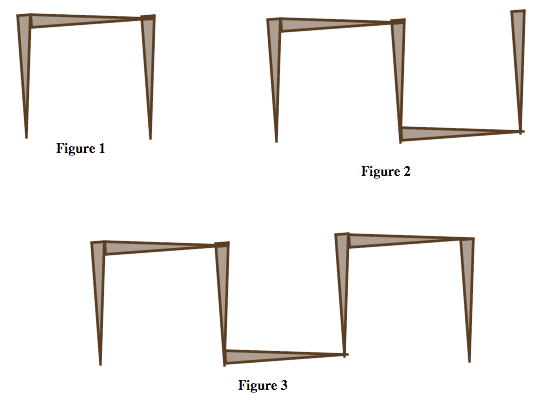
\includegraphics[height=9cm]{toothpicks1}
\end{center}

\end{problem}


\newpage

\begin{problem}\label{prob:toothpics2}\ 

\begin{center}
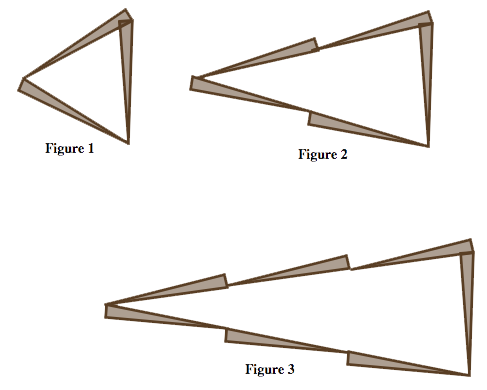
\includegraphics[height=9.5cm]{toothpicks2}
\end{center}

\end{problem}



\bigskip




\begin{problem}\label{prob:toothpics3}\ 

\begin{center}
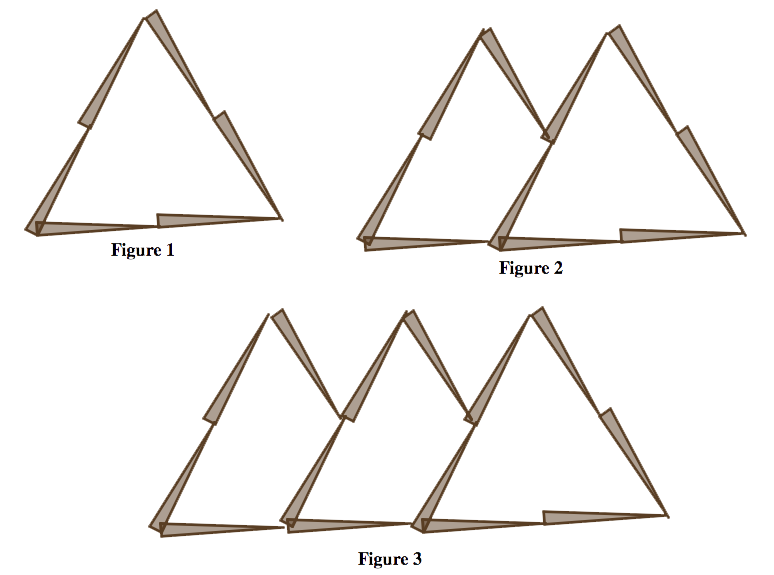
\includegraphics[height=9cm]{toothpicks4}
\end{center}

\end{problem}


\newpage

\bigskip

\begin{problem}\label{prob:toothpics4}\ 

\begin{center}
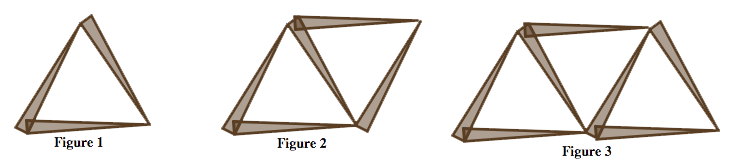
\includegraphics[height=3.5cm]{toothpicks3}
\end{center}

\end{problem}

\newpage


In a \emph{mobile}, the arms must be perfectly balanced for it to hang properly.  The artist Alexander Calder was famous for his artistic mobiles.You can view some of his amazing work at \url{http://calder.org/work/by-category/hanging-mobile}.  Click ``Explore Works.''

\bigskip

Problems~\ref{prob:mobile1}--\ref{prob:mobile2} present you with mobile puzzles.     In these puzzles:
\begin{itemize}
\item
Objects that are the same shape have the same weight.  (So all circles weigh the same, all squares weigh the same, etc.) \\
 \item
Assume the strings and rods that hold the objects together don't factor into the total weight.\\
\item
Each arm of the mobile must have exactly the same weight.
\end{itemize}

\bigskip
\bigskip
\bigskip

\begin{problem}\label{prob:mobile1}
In this puzzle:
\begin{itemize}
\item
The total weight is 36 grams. 
\item
 All shapes weigh less than 10 grams.  
 \item
 All of the weights are whole numbers.
 \item
 One circle weighs more than one square.  
 \end{itemize}
 Find the weight of each piece.  Is there more than one answer?  How do you know you are right?

\begin{center}
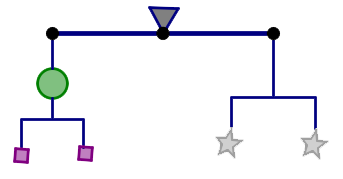
\includegraphics[height=6cm]{mobile1}
\end{center}
\end{problem}

\newpage

\begin{problem}\label{prob:mobile2}
In this puzzle, the total weight is 54 grams.
 Find the weight of each piece.  Is there more than one answer?  How do you know you are right?
\begin{center}
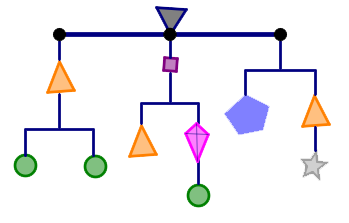
\includegraphics[height=8cm]{mobile2}
\end{center}
\end{problem}




\end{document}
  
